\documentclass{article}
\usepackage{amssymb}
\usepackage[T1]{fontenc}
\usepackage[utf8]{inputenc}
\usepackage{xcolor}
\usepackage{color}
\usepackage{verbatim}
\usepackage{hyperref}
\usepackage{listings}
\usepackage{mathtools}
\usepackage{tikz}
\usetikzlibrary{trees}
\usetikzlibrary{arrows}

\newcounter{questioncounter}
\newcounter{exercisecounter}
\setcounter{questioncounter}{0}
\setcounter{exercisecounter}{0}


% Questions
\newcommand{\question}[1]{
  \refstepcounter{questioncounter}
  \addcontentsline{toc}{subsubsection}{Fråga: 1.\thequestioncounter{} #1}
  \vspace{1em}~
  \\\normalfont{\large{\bfseries{\hspace{0.5em}Fråga 1.\thequestioncounter \hspace{1em}#1}}}\\\\
}

% Exercises
\newcommand{\exercise}[1]{
  \refstepcounter{exercisecounter}
  \addcontentsline{toc}{subsubsection}{Uppgift: 1.\theexercisecounter{} #1}
  \vspace{1em}~
  \\\normalfont{\large{\bfseries{\hspace{0.5em}Uppgift 1.\theexercisecounter \hspace{1em}#1}}}\\\\
}

\lstset{
  language=[Sharp]C,
  basicstyle=\color[rgb]{0.3,0.3,0.3}\ttfamily,
  keywordstyle=\color[rgb]{0,0.5,0.5},
  numberstyle=\color[rgb]{0.7,0.7,0.7},
  commentstyle=\color[rgb]{0.1,0.5,0.1},
  stringstyle=\color[rgb]{0.6,0.1,0.5},
  backgroundcolor=\color[rgb]{0.95,0.95,0.95},
  showstringspaces=false,
  numbers=left,
  breaklines,
  breakatwhitespace,
}
\tikzset{
  treenode/.style = {align=center, inner sep=0pt, text centered,
    font=\sffamily},
  arn_n/.style = {treenode, circle, black, font=\sffamily\bfseries, draw=black,
    text width=1.5em},% arbre rouge noir, noeud noir
  arn_r/.style = {treenode, circle, black, draw=black, 
    text width=1.5em, very thick},% arbre rouge noir, noeud rouge
  arn_x/.style = {treenode, rectangle, draw=black,
    minimum width=0.5em, minimum height=0.5em}% arbre rouge noir, nil
}


\usepackage{tikz}
\usetikzlibrary{trees}




\begin{document}

  \title{Labb III - Träd, heapar och prioriterade köer }
  \author{ Algoritmer och datastrukturer | Uppsala Universitet | VT15 }
  \date{}
  \maketitle


  \section*{Inledning}
 I denna laboration kommer vi att fortsätta att undersöka olika typer av datastrukturer och
 hur de kan nyttjas för att lösa diverse problem. Vi börjar med att undersöka hierarkiska träd
 för att sedan gå vidare till heapar och prioriterade köer.



  \section*{Träd
  }

  Träd är hierarkiska datastrukturer som, till skillnad mot "platta" datastrukturer som t ex
  listor, möjliggör att data struktureras på ett sätt som ger ytterligare mening till innehållet.
  Exempelvis tänk en meny med ett antal undermenyer, vilka i sin tur har egna undermenyer
  o s v. jämför att implementera menyn m.h.a. en hierarkiska trädstruktur eller en platt lista.
  Begrunda exempelvis File-menyn i Visual Studio:\\
  
  \tikzstyle{every node}=[draw=black,thick,anchor=west]
  \tikzstyle{selected}=[draw=red,fill=red!30]
  \tikzstyle{optional}=[dashed,fill=gray!50]
  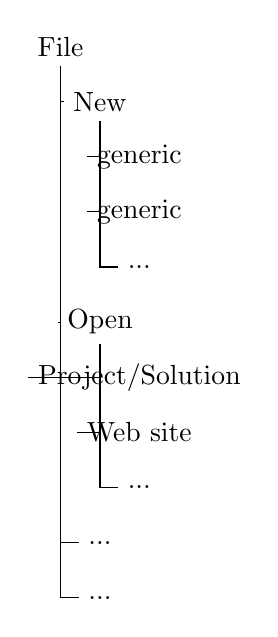
\begin{tikzpicture}[%
    grow via three points={one child at (0.5,-0.7) and
    two children at (0.5,-0.7) and (0.5,-1.4)},
    edge from parent path={(\tikzparentnode.south) |- (\tikzchildnode.west)}]
    \node {File}
      child { node {New}
      		child { node {generic}}
      		child { node {generic}}
      		child { node {...}}		
      		}
      child [missing] {}
      child [missing] {}
      child [missing] {}	
      child { node {Open}
        child { node {Project/Solution}}
        child { node {Web site}}
        child { node {...}}
      }
      child [missing] {}				
      child [missing] {}				
      child [missing] {}				
      child { node {...}}
      child { node {...}};
  \end{tikzpicture}
\\Figuren ovan visar hur vissa menyer blir underordnade andra menyer på grund av valet
av en hierarkiska datastruktur. För en platt datastruktur, exempelvis en lista, hade detta
inte varit möjligt, vilket illustrerar styrkan med ett hierarkiskt upplägg.\\

Begrunda följande träd:
\begin{figure}[h]
\centering
\includegraphics[height=6cm]{graf.png}
\caption{Träd att traversera}
\end{figure}

\begin{enumerate}
\item Traversera trädet i pre-, in- och postorder.
\item Var det någon av traverseringarna som var problematisk att genomföra? Vilken? Varför?
\end{enumerate}

\section*{Binära sökträd - BST}
Binära träd är träd som maximalt kan ha två barn. Då binära träd illustreras, ritas oftadet första barnet åt vänster och det andra barnet åt höger, varvid vi refererar till dem som "vänstra" respektive "högra" barnen. Ett binärt sökträd (Binary Search Tree eller BST) är ett binärt träd som följer en mängd regler gällande inbördes ordning av noder.\\\\

För varje nod N i ett binärt sökträd gäller följande:
\begin{enumerate}
\item Det vänstra barn-trädet innehåller enbart noder med värden mindre än noden N:s
värde.
\item Det högra barn-trädet innehåller enbart noder med värden större än noden N:s värde.
\item Båda barn-träden är binära sökträd.
\end{enumerate}

BST och träd generellt är rekursiva och implementeras med fördel som rekursiva datastrukturer. Ett BST stödjer operationerna Insert, Remove, Find, Inorder, Preorder och Postorder.
Operationer för rekursiva datastrukturer implementeras enklast som rekursiva metoder.
I skalprojektet finns det redan en färdig klass BinareySearchTree<T> som är en så
kallad "wrapper"-klass som kapslar in den rekursiva datastrukturen BinarySearchTre-
eNode<T>. Det är klassen BinarySearchTreeNode<T> som avses i beskrivningen
ovan och det är i den klassen ni senare ska göra er implementation.
Notera att kurslitteraturen inte tar upp denna "wrapper"-klass men det underlättar för er implementation, de förklaringar som avser ett BST i kurslitteraturen avser alltså klassen vi benämner som BinarySearchTreeNode<T>.

\begin{enumerate}
\item Visa hur de rekursiva operationerna Insert, Remove och Find kan fungera genom illustrationer med förklaringar eller genom att skriva pseudokod.
\item Slutför implementationen av klassen BinarySearchTreeNode<T>, implementationen
ska följa det som definierats ovan, både datastrukturen och metoderna skall vara
rekursiva. Vi rekommenderar följande arbetsgång:
\begin{enumerate}
\item Börja med att implementera metoderna Insert och Find. Varje nod i det binära
sökträdet ska innehålla tre referenser till andra noder, två av dessa till sina barn
och en till sin förälder
\item Fortsätt med att implementera metoden Remove, remove-algoritmen bygger på
att referenserna till barn och förälder är korrekta. Tänk på att dessa referenser
även måste uppdateras när en nod tas bort ur trädet.
\item När ni har testat att ni kan lägga till, ta bort och leta efter värden i ert träd går ni vidare med att implementera traverseringsmetoderna.
\end{enumerate}
\item Uppdatera ditt gränssnitt (GUI) så att det stödjer operationerna Insert, Remove och Find för ett BST, trädets pre-, in- och postorder skall hela tiden vara presenterade.
\end{enumerate}



  \section*{Heapar
  }
  
  En min-heap är en trädstruktur där varje föräldernod har ett värde som är mindre än sina barn. Alltså har rotnoden det minsta värdet. I en max-heap är det tvärtom, dvs rotnoden har det största värdet och varje föräldernod har ett värde som är större än sina barn. En heap implementeras oftast med en platt datastruktur, t ex en array, och har samma begränsning som binära träd gällande antalet barn. Varje nod kan därför endast ha två barn.
  För att kunna implementera en hierarkisk struktur i en array krävs regler som dikterar hur vi kan identifiera barn- och föräldernoder för en given nod. Följande strategi, som inte är specifik för just en heap utan även kan nyttjas för att representera ett binärt träd i en array, används:
  
  \begin{figure}[h]
  \centering
  \includegraphics[height=3cm]{x.png}
    \end{figure}
  \begin{enumerate}
  \item En min-heap har följande underliggande array: [2, 6, 8, 16, 9, 10]. Representera heapen som ett träd på papper.
  \item Illustrera varje steg på papper när du lägger in talen 7, 2, 18, 32, 4, 1, 10 och 12 i en  min-heap och sedan tar bort 4 och 7.
  \item Gör en implementation av en min-heap i klassen MinHeap<T> som stöder operationerna Add och Remove. Låt klassen ha en konstruktor som initerar en tom heap med en given kapacitet.
  \item Uppdatera ditt gräanssnitt så att det stödjer operationerna Add och Remove för en minheap. Omdefiniera ToString-metoden så att du enkelt kan presentera hela heapen i ditt
  GUI.
  \end{enumerate}
 
\end{document}